\section{Application to Model Selection for Primal SVM}

\textcolor{red}{Skalarprodukt anpassen, Vektoren nicht fett oder neue definition, notation, \(\lambda \in \Lambda\) einfugen\\
Vektoren (in gesamter Arbeit) in runden Klammern}

\subsection{Introduction}

In this part of the thesis the nonconvex inexact bundle algorithm \textcolor{red}{number in thesis} is applied to the problem of model selection for \emph{support vector machines} (SVMs) solving classification tasks.
It relies on a bilevel formulation proposed by Kunapuli in \cite{Kunapuli2008} and Moore et al. in \cite{Moore2011}.

A natural application for the inexact bundle algorithm is an optimization problem where the objective function value and subgradient can only be computed by numerical approximation. This is for example the case in bilevel optimization.
%If this objective function is iteratively optimized, the function value i never exact. But by the stopping condition it is (often???) possible to have the needed error bound on the function value (what about the gradient???). (Comment on asymptotical exactness?)

%A general bilevel problem can be formulated as 
%Bilevel optimization deals with a class of constrained optimization problems where one or more of the optimization variables are again constrained by optimization problems.
A general bilevel program can be formulated as in \cite[p. 20]{Kunapuli2008}

\begin{equation}
	\begin{array}{cll}
	\displaystyle\min_{C \in U_{ad}, \tilde{w} \in \R^k} & \mathcal{L}_{upp}(C,\tilde{w}) & \text{upper level} \vspace{0.5ex}\\
	\text{s.t.} & \mathcal{G}_{upp}(C,\tilde{w}) \leq 0 & \vspace{1em}\\
	& \tilde{w} \in \begin{Bmatrix} \displaystyle\argmax_{\tilde{w}\in W} & \mathcal{L}_{low}(C,\tilde{w}) \vspace{0.5ex}\\
	                        \text{s.t.} & \mathcal{G}_{low}(C,\tilde{w}) \leq 0 
													\end{Bmatrix}. & \text{lower level}
	\end{array}
	\label{bilevel}
\end{equation}

The two objecective functions \(\mathcal{L}_{upp}\) and \(\mathcal{L}_{low}\) map from \(\R^n\times\R^k\) into \(\R\) and the constraint functions \(\mathcal{G}_{upp}\) and \(\mathcal{G}_{low}\) map from \(\R^n\times\R^k\) into \(\R^l\) and \(\R^s\) respectively. 

The problem consists of an \emph{upper} or \emph{outer level} which is the overall function to be optimized. Contrary to usual constrained optimization problems which are constrained by explicitly given equalities and inequalities a  bilevel program is additionally constrained by a second optimization problem, the \emph{lower} or \emph{inner level} problem.

Solving bilevel problems can be divided roughly in two classes: implicit and explicit solution methods. 
In the explicit methods the lower level problem is usually rewritten by its KKT conditions, these are then added as constraints to the upper level problem. With this solution method the upper and lower level are solved simultaneously. For the setting of model selection for support vector machines as it is used here, this method is described in detail in \cite{Kunapuli2008}.

The second approach is the implicit one. Here the lower level problem is solved directly in every iteration of the outer optimization algorithm and the solution is plugged into the upper level objective. 

Obviously if the inner level problem is solved numerically, the solution cannot be exact. Additionally the \emph{solution map} \( S(C) = \{w\in \R^k \mid w\) solves the lower level problem for a given \(C\}\), can be nondifferentiable \cite{Outrata1998} and since elements of  the solution map are plugged into the outer level objective function in the implicit approach, the outer level function then becomes nonsmooth itself. This is why the inexact bundle algorithm seems a natural choice to tackle these bilevel problems. 

Moore et al. use the implicit approach in \cite{Moore2011} for support vector regression. However they use a gradient descent method which is not guaranteed to stop at an optimal solution.
In \cite{Moore2010a} it is also suggested to use the nonconvex exact bundle algorithm of Fuduli et al. \cite{Fuduli2004a} for solving the bilevel regression problem. This method allows for nonsmooth inner problems and can theoretically solve some of the issues of the gradient descent method. It ignores however, that the objective function values can only be calculated approximately. A fact which is not addressed in Fuduli's algorithm.

%\subsection{Notation and Expressions}

%training set, validation /holdout set...

\subsection{Notation}

As short remark on the notation in this chapter is required.

Due to standard notation in the field of SVM, the variables \(x\) and \(y\) are used in this chapter in a different manner than before.
%In the setting of bilevel problems as used in (\ref{bilevel}) \(x \in X \subset \R^n\) and \(y \in \R^k\) are the optimization variables of the bilevel problem.

In the setting of SVMs \(x^i \in \R^{n_f}\) is an element of the \emph{feature space} that contains the values of one data point. The corresponding variable \(y_i \in \{-1,1\}\) of the \emph{output domain} contains the class in which the data point \(x^i\) lies. Sometimes the indices of the samples are omitted to express the general dependency on the data (x,y).
%All samples can be wrapped up in a martix \(X \in \R^{feat\times nd}\) and a vector \(Y\in \R^{nd}\).
The optimization variable of the bundle method is denoted by \(C\) during this chapter.

%During the most part of the chapter, \(x^i\) and \(y^i\) are used as in the context of SVMs. In the cases where they are used to describe the variables of an optimization problem, this is clearly indicated.

There appear also different derivatives in this chapter.
For a continuously differentiable function \(f:\R^n \times \R^k \to \R\) we denote the \emph{gradient} at \((\bar{C},\bar{\tilde{w}})\) by \(\nabla f(\bar{C},\bar{\tilde{w}}) \in \R^{n+k}\). The partial gradient with respect to \(\tilde{w}\) is indicated by \(\nabla_{\tilde{w}}f(\bar{C},\bar{\tilde{w}}) \in \R^k \). %If \(f\) is twice continuously differentiable the \emph{Hessian matrix} at the point \((\bar{x},\bar{y})\) is given by \(\nabla^2 f(\bar{x},\bar{y}) \in \R^{n+m \times n+m}\).
For a continuously differentiable vector valued function \(F:\R^n \times \R^k \to \R^m\) the \emph{Jacobian matrix} is given by \( \mathcal{J}F(\bar{C},\bar{\tilde{w}}) \in \R^{m \times (n+k)}\). The partial Jacobian with respect to the variable \(\tilde{w}\) is denoted \(\mathcal{J}_{\tilde{w}} F(\bar{C},\bar{\tilde{w}}) \in \R^{m \times k}\).

Finally let \(M \in \R^{n\times k}\) be a matrix and \(I \subset \{1,...,n\}\) an index set. Then the expression \(M_{I}\) denotes the matrix that consists of the rows of \(M\) corresponding to the indices in the set \(I\). %For a vector \(v \in \R^n\) the vector \(v_{I}\) consists of the components of \(v\) corresponding to the set \(I\).

%special notation only in this chapter, \(x,y\) now different. Optimization variable now \(\lambda,C\).
%with index -> data, without variables from problem.
%Will be clear from context.
%
%do this due to the standard notation in the field of SVM

\subsection{Introduction to Support Vector Machines}
%In times of big data machine learning is a very active field of research. 
Support vector machines are linear learning machines that were developed in the 1990's by Vapnik and co-workers (see \cite{Boser1992}, where SWMs were introduced). Soon they could outperform several other programs in this area \cite{Cristianini2000} and the subsequent interest in SVMs led to a very versatile application of these machines \cite{Kunapuli2008}.

The case that is considered here is binary support vector classification using supervised learning. 
For a throughout introduction to this subject see also \cite{Cristianini2000}. Here a summary of the most important expressions and results is given.

In classification data from a possibly high dimensional vector space \(\tilde{X} \subset \R^{n_f}\), the feature or \emph{input space} is divided into two classes. These lie in the output domain \(\tilde{Y} = \{-1,1\}\). Elements from the feature space will mostly be called \emph{data points} here. They get \emph{labels} from the feature space. Labeled data points are called \emph{examples}.
The functional relation between the features and the class of an example is given by the usually unknown \emph{response} or \emph{target function} \(f(x)\).
Supervised learning is a kind of machine learning task where the machine is given examples of input data with associated labels, the so called \emph{training data} \((X,Y)\). Mathematically this can be modeled by assuming that the examples are  drawn \emph{identically and independently distributed} (iid) from the fixed joint distribution \(P(x,y)\). This usually unknown distribution states the probability that a data point \(x\) has the label \(y\) \cite[p. 988]{Vapnik1999}.
The overall goal is then to optimize the generalization ability, meaning the ability to predict the output for unseen data correctly \cite[chapter 1.2]{Cristianini2000}.
%The overall goal of machine learning is to optimize the generalization ability of the algorithm --> this means: predict output for unlabeled input as well as possible.
%task is to find a mapping that predicts the output given unlabeled input as good as possible \cite{Cristianini2000}. 

\subsubsection{Risk minimization}
The concept of SVM's was originally inspired by the statistical learning theory developed by Vapnik. A detailed examination of the subject is given in \cite{Vapnik1998}. In \cite{Vapnik2013} the subject is approached from a more explaining point of view.

%from: Vapnik - Statistical Learning Theory overview \cite{Vapnik1998}
The idea of \emph{risk minimization} is to find from a fixed set or class of functions the one that is the best approximation to the response function. This is done by minimizing a loss function that compares the given labels of the examples to the response of the learning machine.
%goal: find best available (from set of functions that was chosen before) approximation to the actual (unknown) ``response function'' --> function that ``classifies'' the data
%Minimize loss between response of ``supervisor'' and response of learning machine

As the response function is not known, only the expected value of the loss can be calculated. It is given by the \emph{risk functional} 

\begin{equation}
	R(\lambda) = \int{\mathcal{L}(y,f_{\lambda}(x))\text{d}P(x,y)}.
\label{risk_func}
\end{equation}

Here \(\mathcal{L}: \R^2 \to \R\) is the loss function, \(f_{\lambda}: \R^{n_f} \to \R, ~ \lambda \in \Lambda\) the approximate response function found by the learning machine and \(P(x,y)\) the joint distribution the training data is drawn from. The goal is now to find a function \(f_{\bar{\lambda}}(x)\) in a chosen function space \(\mathcal{F}\) that minimizes this risk functional \cite[p. 989]{Vapnik1999}.

As the only given information is provided by the training set inductive principles are used to work with the \emph{empirical risk}, rather than with the risk functional.
The empirical risk only depends on the finite training set  and is given by 

%goal: find \(f_{\lambda_0}(x)\) that minimizes this functional
%\(P(x,y)\) is unknown
%Because only a data sample is known: Work with the empirical risk

\begin{equation}
	R_{\text{emp}}(\lambda) = \frac{1}{n_d} \sum_{i = 1}^{n_d}\mathcal{L}(y_i,f_{\lambda}(x^i)),
\label{emp_risk}
\end{equation}

where \(n_d\) is the number of data points.
%L: Loss function 
%Goal: approximate \(Q(z,\lambda_0)\) by \(Q(z,\lambda_l)\) that minimizes the empirical risk. --> is called ERM (empirical risk minimization induction principle)
The law of large numbers ensures that the empirical risk converges to the risk functional as the number of data points grows to infinity. This however does not guarantee that the function \(f_{\bar{\lambda},\text{emp}}\) that minimizes the empirical risk also converges towards the function \(f_{\bar{\lambda}}\) that minimizes the risk functional.
The theory of consistency provides necessary and sufficient conditions that solve this issue  \cite[p. 989]{Vapnik1999}.

Vapnik therefore introduced the structural risk minimization (SRM) induction principle. It ensures that the used set of functions has a structure that makes it strongly consistent \cite{Vapnik1999}. Additionally it takes the complexity of the function that is used to approximate the target function into account. ``The SRM principle actually suggests a tradeoff between the quality of the approximation and the complexity of the approximating function'' \cite[p. 994]{Vapnik1999}.
This reduces the risk of \emph{overfitting}, meaning to overly fit the function to the training data with the result of poor generalization \cite[chapter 1.3]{Cristianini2000}.

%Therefore: structural risk Minimization induction Principle (SRM) --> is strongly consistent --> idea: minimize the empirical risk by considering the complexity of the model (given by CV-dimension)

Support vector machines fulfill all conditions of the SRM principle. Due to the kernel trick that allows for nonlinear classification tasks it is also very powerful. For more detailed information on this see \cite{Kunapuli2008} and references therein.

\subsubsection{Support Vector Machines}

In the case of linear binary classification one searches for a an affine hyperplane \(w \in \R^{n_f}\) shifted by \(b \in \R\) to separate the given data. The vector \(w\) is called weight vector and \(b\) is the bias.

Let the data be linearly separable. This means, that there exists an affine hyperplane \((w,b)\) such that all data points from one class are on the same side of the hyperplane. The function deciding how the data is classified can be written as

\[ f(x) = \text{sign}(\Langle w,x\Rangle-b). \]

Support vector machines aim at finding such a hyperplane that separates also unseen data optimally.

\textcolor{red}{???Picture of hyperplane}

One problem of this approach is that the representation of a hyperplane is not unique. If the plane described by \((w,b)\) separates the data, there exist infinitely many hyperplanes \((tw,b)\), \(t>0\), that separate the data in the same way.
To have a unique description of a separating hyperplane the \emph{canonical hyperplane for given data} \(x \in X\) is defined by 

\[ f(x) = \Langle w, x\Rangle - b  \quad \text{s.t.} \quad \min_i \vert\Langle w,x^i\Rangle -b\vert = 1.\] 

To find such a hyperplane is always possible in the case where the data is  linearly separable. It means that the inverse of the norm of the weight vector is equal to the distance of the closest point \(x \in X \) to  the hyperplane \cite[p. 10]{Kunapuli2008}.


%Kunapuli: representation of hyperplane not unique --> if \((w,b)\) separates data, infinitely many hyperplanes \((tw,tb) \forall t > 0\) also separate data --> need unique representation --> w.l.o.g. define \emph{canonical hyperplane} for given data \(x \in X\) as function 
%only valid for separable data

This gives rise to the following definition:
The \emph{margin} is the minimal Euclidean distance between a training example \(x^i\) and the separating hyperplane.
%one can show that margin invese proportional to norm of \(w\).
A bigger margin means a lower complexity of the function \cite{Cristianini2000}. 

A \emph{maximal margin hyperplane} is the hyperplane that realizes the maximal possible margin for a given data set.

%Theorem 6.1
\begin{proposition}[{\cite[Proposition 6.1]{Cristianini2000}}]
Given a linearly separable training sample \ \(\Omega = \{(x^1,y_1),...,(x^{n_d},y_{n_d})\}\) the hyperplane \((w,b)\) that solves the optimization problem

\[\|w\|^2 \quad \text{s.t.} \quad y_i(\Langle w,x^i\Rangle-b)\geq 1, \quad i = 1,...,n_d, \]

realizes a maximal margin hyperplane.
\end{proposition}

The proof is given in \cite[chapter 6.1]{Cristianini2000}. 

Generally one cannot assume the data to be linearly separable. This is why in most applications a so called \emph{soft margin classifier} is used. It introduces the slack variables \(\xi_i\) that measure the distance of the misclassified points to the hyperplane:

%from this follows: soft margin classifyer --> not any more assumption that data linearly separable --> slack variables \(\xi_i\) measure the distance of misclassified points

%Def 2.6:
%\begin{definition} \cite{Cristianini2000}
Fix \(\gamma > 0\). A \emph{margin slack variable of the example} \((x^i,y_i)\) with respect to the hyperplane \((w,b)\) and target margin \(\gamma\) is 

\[\xi_i = \max(0, \gamma - y_i(\Langle w,x^i\Rangle+b))\] 

%\end{definition}  
If \(\xi_i > \gamma\) the point is considered misclassified. 
One can also say that \(\|\xi\|\) ``measures the amount by which the training set fails to have margin \(\gamma\)'' \cite[section 2.1.1]{Cristianini2000}.

For support vector machines the target margin is set to \(\gamma = 1\).

%Book uses \(\xi^2\) -> then \(\xi>0\) not needed any more; only \(\xi\) also used -> 1-norm
%This results finally in the following slightly different
%optimization problems for finding an optimal separating hyperplane \((w,b)\):

This results in the following optimization problem for finding an optimal separating hyperplane \((w,b)\): 


%and
%
\begin{align}
\begin{split}
	\min_{w,b,\xi} \quad & \frac{1}{2} \|w\|^2_2+\frac{C}{2}\sum_{i=1}^{n_d}{\xi_i^2} \vspace{0.5ex}\\
	\text{s.t.} \quad & y_i\left(\Langle w,x^i\Rangle-b\right) \geq 1 - \xi_i \vspace{0.5ex}\\
	& 	\forall i = 1, \dots , n_d.
\end{split}
\label{SVM_2}
\end{align}

%The first part of the respective objective functions are the regularizations, the second part are the actual loss functions.
The first part of the objective function is the regularization, the second part the actual loss function. 
The parameter \(C > 0\) gives a trade-off between the richness of the chosen set of functions \(f_{\lambda}\) to reduce the error on the training data and the danger of overfitting to have good generalization. It has to be chosen a priori \cite{Kunapuli2008}.
%The two optimization problems only differ in the norm chosen for the loss function. In (\ref{SVM_1}) the one-norm is chosen, in (\ref{SVM_2}) the squared two-norm is used.

Instead of the Euclidean norm it is also possible to use the 1-norm in the loss function. Then the resulting optimization problem reads

\begin{align*}
\begin{split}
	\min_{w,b,\xi} \quad & \frac{1}{2} \|w\|^2+C\sum_{i=1}^{n_d}{\xi_i} \\
	\text{s.t.} \quad & y_i\left(\Langle w,x^i\Rangle-b\right) \geq 1 - \xi_i \\
	& \xi_i \geq 0 \\
	& 	\forall i = 1, \dots , n_d.
\end{split}
%\label{SVM_1}
\end{align*}

In this form, however, the problem does not fit the theory described in \cite{Outrata1998}, which is used later to solve the constructed bilevel problem. \textcolor{red}{refer to appendix were counterexample to strong regularity is given?\\
It is shown in appendix ... that there exist data sets for which the strong regularity condition stated in ... is violated. Thus the subgradient of the upper level objective function cannot be calculated as proposed in \cite{Outrata1998}.}


%To derive a subgradient of the bilevel problem introduced later in this section another formulation of the classification problem is used.
In order to fulfill all conditions assumed in \cite{Outrata1998} it is necessary to reformulate problem (\ref{SVM_2}).
The new formulation makes use of the \emph{implicit bias}, meaning that the bias is not calculated separately but as part of the variable \(w\). 
By adding an additional '1' to the end of each feature vector we can use the vectors \(\tilde{x}_i := (x_i^{\top},1)^{\top}\) and \(\tilde{w} := (w^{\top},w_b)^{\top}\) to state the following optimization problem:

\begin{align}
\begin{split}
	\min_{\tilde{w},\xi} \quad & \frac{1}{2} \|\tilde{w}\|^2+\frac{C}{2}\sum_{i=1}^{n_d}{\xi_i^2} \vspace{0.5ex}\\
	\text{s.t.} \quad & y_i\Langle \tilde{w},\tilde{x}^i\Rangle = y_i\left(\Langle w,x^i\Rangle-w_b\right) \geq 1 - \xi_i \vspace{0.5ex}\\
	& 	\forall i = 1, \dots , n_d.
\end{split}
\label{SVM_bias}
\end{align}

Not treating the bias separately is a strategy used for example to achieve a more efficient implementation \cite[section 3.2, p. 22]{Gunn1998}. In the course of this section the gain of this particular formulation is the fact that it has a unique solution \textcolor{red}{compare for... where it is shown}.
It is however shown in \cite[section 3.2, p. 22]{Gunn1998} that the solutions that are found with explicit and implicit bias are different.
This results from the fact that in case of implicit bias the variable \(b\) also enters the regularization term.

From now on we work with the implicit bias. To see the derivation of the bilevel problem with the explicit bias compare for \cite[section 2.2]{Kunapuli2008}.

\subsubsection{Multiple Hyper-parameters}

To examine the performance of the bilevel approach in the more dimensional case a model suggested by Moore et al. in \cite{Moore2011} called \emph{multi-group} support vector classification (multiSVC) is used. This model allows different hyper-parameters for different subgroups of the trainings data.
In section 4.3 of \cite{Moore2011} the model is described for a regression function. In this thesis the same technique is used for classification.

The motivation behind the approach is that different groups of samples from the training set can have slightly different properties and should therefore have their own weighting parameters \(C_g\).
On the one hand this can improve the generalization results. On the other hand properties of the different data groups can be identified by their respective hyper-parameters. Moore et al. explain in \cite[section 4.3, p. 9]{Moore2011} that for example a large value of \(C_g\) signifies reliable data in the respective group whereas a smaller \(C_g\) suggests a poorer quality.

To perform multiSVC, divide the trainings data into \(G\) (pairwise disjoint) groups.
Define the vector of hyper-parameters \(C := (C_1,...,C_G)^{\top}\). For the sake of simplicity in this thesis all the groups are of equal size but all derivations are also possible for differently sized groups.

%For \(T\)-fold cross validation the \(t\)'th 
The multi-group classification problem in constrained form can be stated as 

\begin{align}
\begin{split}
	\min_{\tilde{w},\xi} \quad & \frac{1}{2} \|\tilde{w}\|^2+\sum_{g = 1}^G\left(\frac{C_g}{2}\sum_{i \in N_g} {\xi_i^2}\right) \vspace{0.5ex}\\
	\text{s.t.} \quad & y_i\Langle \tilde{w},\tilde{x}^i\Rangle \geq 1 - \xi_i \vspace{0.5ex}\\
	& 	\forall i \in \bigcup_{g =1}^G N_g =\{1,...,n_d\}.
\end{split}
\label{MultiSVC_QP}
\end{align}

Here \(N_g\) is the index set that contains the indices of the data of the \(g\)'th group.


\subsection{Formulation of the Bilevel Problem}
%Check if regression case also included?????

%\textcolor{red}{adapt all section titles -> introduction of MultiGroup}

The hyper-parameters \(C_g\) in the objective function of the classification problem have to be set beforehand. This step is part of the model selection process.
To set the parameters optimally different methods can be used.
A very intuitive and widely used approach is doing \emph{cross validation} (CV) with a grid search implementation \cite[p. 30]{Kunapuli2008}.
%very costly, discrete parameter choice, not practicable in case of many parameter

To prevent overfitting and get a good parameter selection, especially in case of little data, commonly \(T\)-fold cross validation is used \cite[p. 30]{Kunapuli2008}.
For this technique the training data is randomly partitioned into \(T\) subsets of equal size. One of these subsets is then left out of the training set and instead used afterwards to get an estimate of the generalization error. 
To use CV for model selection it has to be embedded into an optimization algorithm over the hyper-parameter space. 
Commonly this is done by discretizing the parameter space and for \(T\)-fold CV training \(T\) models at each grid point. The resulting models are then compared to find the best parameters in the grid.
Obviously for a growing number of hyper-parameters this is very costly. An additional drawback is that the parameters are only chosen from a finite set \cite[p. 30]{Kunapuli2008}.

%\subsubsection{Reformulation as Bilevel Problem}

A more recent approach is the formulation as a bilevel problem used in \cite{Kunapuli2008} and \cite{Moore2011}.
This makes it possible to optimize the hyper-parameters continuously.

%Formal description of the bilevel problem for t-fold cross validation
%Better model description --> see 2.2 (p.46) in thesis 

Let \(\Omega = \{(x^1,y_1),...,(x^{n_d},y_{n_d})\} \subset \R^{n_f+1}\) be a given data set of size \(n_d = |\Omega|\). The associated index set is denoted by \(\mathcal{N}\). For classification the labels \(y_i\) are \(\pm1\).
For \(T\)-fold cross validation let \(\bar{\Omega}_t\) and \(\Omega_t\) be the training set and the validation set respectively within the \(t\)'th fold and \(\bar{\mathcal{N}}_t\) and \(\mathcal{N}_t\) the respective index sets. For multi-group SVC the index set \(\bar{\mathcal{N}}_t\) is again divided into the \(G\) sets \(\bar{\mathcal{N}}_t^g\) to account for the different groups associated with the different hyper-parameters.
Furthermore let \(f^t:\R^{n_f+1} \to \R\) be the response function trained on the \(t\)'th fold and \(\lambda \in \Lambda\) the hyper-parameter to be optimized.
For a general machine learning problem with upper and lower loss function \(\mathcal{L}_{upp}\) and \(\mathcal{L}_{low}\) respectively the bilevel problem reads
 
%%% introduce \mathcal(F) already before as the function space

\begin{equation*}
	\begin{array}{cll}
	\displaystyle\min_{\lambda, f^t} & \mathcal{L}_{upp}\left(\lambda,f^1|_{\Omega_1},...,f^T|_{\Omega_T}\right) & \text{upper level} \vspace{0.5ex}\\
	\text{s.t.} & \lambda \in \Lambda & \vspace{1em}\\
	& \text{for } t = 1,...,T: & \\
	& f^t \in \begin{Bmatrix} \displaystyle\argmin_{f\in \mathcal{F}} & \mathcal{L}_{low}(\lambda,f,(x^i,y_i)_{i = 1}^l\in \bar{\Omega}_t) \vspace{0.5ex}\\
	                        \text{s.t.} & \mathcal{G}_{low}(\lambda,f) \leq 0 
													\end{Bmatrix}. & \text{lower level}
	\end{array}
\end{equation*}

In the case of multigroup support vector classification the \(T\) inner problems have the SVM formulation %(\ref{SVM_1}) or 
(\ref{MultiSVC_QP}). % (but all \(T\) problems have the same formulation).
This problem can also be rewritten into an unconstrained form. It is helpful when using the inexact bundle algorithm for solving the bilevel problem.
For the \(t\)'th fold the resulting hyperplane is identified with the variable \(\tilde{w}^t \in \R^{n_f+1}\).
The inner level problem for the \(t\)'th fold can therefore be stated as

%\begin{equation}
	%(w^t,b_t) \in \argmin_{w,b}\left\{ \frac{\lambda}{2} \|w\|^2_2+\sum_{i\in \bar{\mathcal{N}}_t}{\max\left(1-y_i(w^{\top}x^i-b),0\right)}\right\}
%\label{lower_t_1}
%\end{equation}

%or

\begin{equation}
	\tilde{w}^t \in \argmin_{\tilde{w}} \left\{\frac{1}{2} \|\tilde{w}\|^2+\sum_{g=1}^G\left(\frac{C_g}{2}\sum_{i\in \bar{\mathcal{N}}_t^g}{\max\left\{1-y_i\Langle \tilde{w},\tilde{x}^i\Rangle,0\right\}^2}\right)\right\}.
\label{lower_unconstr}
\end{equation}

%Where the hyper-parameter \(\lambda = \frac{1}{C}\) is used  due to numerical stability \cite[p. 38]{Kunapuli2008}.

For the upper level objective function different choices are possible. All that are presented here use the implicit bias. They all can also be used with the explicit bias term.

Simply put, the outer level objective should compare the different inner level solutions and pick the best one. An intuitive choice is therefore to pick the misclassification loss, that counts how many data points of the respective validation set \(\Omega_t\) are misclassified when taking function \(f^t\).

The misclassification loss can be written as

\begin{equation}
	\mathcal{L}_{mis}(\tilde{w}) = \frac{1}{T}\sum_{t=1}^T\frac{1}{|\mathcal{N}_t|}\sum_{i \in \mathcal{N}_t}{\left(-y_i\Langle \tilde{w}^t,\tilde{x}^i\Rangle\right)_{\star}},
\label{misclass_loss}
\end{equation}

where the step function \((\cdot)_{\star}\) is defined component wise for a vector as
\begin{equation}
	(r_{\star})_i = \left\{\begin{array}{c} 1, \quad \text{if } r_i > 0, \\ 0, \quad \text{if } r_i \leq 0 \end{array} \right. .
\label{step_fun}
\end{equation}

The drawback of this simple loss function is that it is not continuous and thus not suitable for subgradient based optimization. Therefore another loss function is used for the upper level problem, the \emph{hinge loss} or \emph{L1-loss}. It is an upper bound on the misclassification loss and reads

\begin{equation}
		\mathcal{L}_{hinge}(\tilde{w}) = \frac{1}{T}\sum_{t=1}^T\frac{1}{|\mathcal{N}_t|}\sum_{i \in \mathcal{N}_t}{\max\left\{1-y_i\Langle \tilde{w}^t,\tilde{x}^i\Rangle,0\right\}}.
\label{hinge_loss}
\end{equation}

It is also possible to square the max term. This results in the \emph{L2-loss} function

\begin{equation}
		\mathcal{L}_{hingequad}(\tilde{w}) = \frac{1}{T}\sum_{t=1}^T\frac{1}{|\mathcal{N}_t|}\sum_{i \in \mathcal{N}_t}{\max\left\{1-y_i\Langle \tilde{w}^t,\tilde{x}^i\Rangle,0\right\}^2}.
\label{hingequad_loss}
\end{equation}

We refer to this second loss function also as \emph{hingequad loss}.

%In figure (\ref{??}) it can be seen that its minimum and overall progress is more similar to the misclassification loss than the one of the hinge loss. 
%\textcolor{red}{For this reason we progress taking the squared form of the hinge loss, abbreviating with \emph{hingequad loss} for convenience.\\
%No, take hingeloss because of nonsmoothness}

%\textcolor{red}{also possible to square the max term\\
%formula \\
%from plots: seems to match the misclassification loss a bit better -> used it instead/also}

For the bilevel problem discussed in this thesis the hingequad function is chosen as objective of the upper level problem.
Hence the final resulting bilevel formulation for model selection in multigroup support vector classification is 

%\begin{align}
%\begin{split}
	%\min_{w,\bm{b}} \quad &  \mathcal{L}_{hinge}(w,\bm{b}) = \frac{1}{T}\sum_{t=1}^T\frac{1}{|\mathcal{N}_t|}\sum_{i \in \mathcal{N}_t}{\max\left(1-y_i((w^t)^{\top}x-b_t),0\right)}\\
	%\text{subject to} \quad &  \lambda > 0 \\
	%& \text{for } t = 1,...,T \\
	%& (w^t,b_t) \in \argmin_{w,b}\left\{ \frac{\lambda}{2} \|w\|^2_2+\sum_{i\in \bar{\mathcal{N}}_t}{\max\left(1-y_i(w^{\top}x^i-b),0\right)}\right\} \\
%\end{split}
%\label{model_1}
%\end{align}
%
%and 

\begin{align}
\begin{split}
	\min_{C} \quad &  \mathcal{L}_{hingequad}(\tilde{w}) = \frac{1}{T}\sum_{t=1}^T\frac{1}{|\mathcal{N}_t|}\sum_{i \in \mathcal{N}_t}{\max\left\{1-y_i\Langle \tilde{w}^t,\tilde{x}^i\Rangle,0\right\}^2}\\
	\text{s.t.} \quad & C := (C_1,...,C_G) > 0 \\
	& \text{for } t = 1,...,T \\
	& \tilde{w}^t \in \argmin_{\tilde{w}}\left\{ \frac{1}{2} \|\tilde{w}\|^2+\sum_{g=1}^G\left(\frac{C_g}{2}\sum_{i\in \bar{\mathcal{N}}_t^g}\max\left\{1-y_i\Langle \tilde{w},\tilde{x}^i\Rangle,0\right\}^2\right)\right\}. \\
\end{split}
\label{bilevel_fin}
\end{align}

Obviously this bilevel problem contains the usual support vector classification with only one data group as a special case.


%%%%%%%%%%%%%%%%%%%%%%%%%%%%%%%%%%%%%%%%%%%%%%%%%%%%%%%%%%%%%%%%%%%%%%%%%%%%%%%%%
%Here \(\bar{\mathcal{N}}_t^g\) the index set that contains the indices of the data in the \(g\)'th group of the \(t\)'th fold.
%
%Reformulation of the lower level objective:
%
%\begin{equation*}
	%\mathcal{L}_{low}(w,b) =  \frac{1}{2} \|w\|^2+\sum_{g = 1}^GC_g\left(\sum_{i\in \bar{\mathcal{N}}_t^g}\max\left\{1-y_i\left(\Langle w,x^i\Rangle-b\right),0\right\}^2\right)
%\label{ll_mult_group}
%\end{equation*}

%\begin{align*}
	%\min_{w,b,\xi} \quad & \frac{1}{2} \|w\|^2_2+\sum_{g = 1}^G\left(C_g\sum_{i \in \bar{\mathcal{N}}_t^g}{\xi_i^2}\right) \vspace{0.5ex}\\
	%\text{s.t.} \quad & y_i\left(\Langle w,x^i\Rangle-b\right) \geq 1 - \xi_i \vspace{0.5ex}\\
	%& 	\forall i \in \bigcup_{g =1}^G \bar{\mathcal{N}}_t^g = \bar{\mathcal{N}}_t
%\label{MultiSVM_QP}
%\end{align*}
%
%the \(\mathcal{N}_t^g\) are pairwise disjoint

%\(w \in \R^n, b\in \R, \xi \in \R^{\vert\bar{\mathcal{N}}_t \vert}\)




\subsection{Solution with the Inexact Bundle Algorithm}

\textcolor{red}{more introduction?}

The bilevel problem (\ref{bilevel_fin}) derived above is to be solved with the bundle algorithm \textcolor{red}{which one? more?}.
This requires having in every iteration an approximate value of the upper level objective function and an approximate subgradient of the upper level objective.

To understand the issues arising when computing especially the subgradient of a bilevel objective consider again the general bilevel problem (\ref{bilevel}).

At the current iterate \(C^k\) the function value of the upper level objective function can be computed by solving the lower level problem given \(C^k\).
The resulting solution \(\tilde{w}^k = (\tilde{w}^{1,k},...,\tilde{w}^{T,k})\) is then inserted into the upper level objective and its value can be calculated.

For computing a subgradient, it is not that simple. Additionally to the variation of the upper level function \(\mathcal{L}_{upp}\) with respect to the variable \(\tilde{w}\) also the variation of the solution \(\tilde{w}^k\) with respect to \(C\) has to be considered.
To do this we follow the strategy described in \cite{Outrata1998}. Refer there also for a more throughout analysis on this subject.

\subsubsection{Assumptions}

Consider the general bilevel problem formulation (\ref{bilevel}) without the explicit constraint \(\mathcal{G}_{upp}(C,\tilde{w}) \leq 0\).
Let the feasible set \(U_{ad}\) be a nonempty compact set and \(\tilde{A}\) an open set containing \(U_{ad}\).
To use the implicit programming approach suggested in \cite{Outrata1998},  the following assumptions have to hold true:

\begin{itemize}
\item[(A1)] The upper level objective \(\mathcal{L}_{upp}\) is continuously differentiable on \(\tilde{A}\times \R^k\).
\item[(A2)] The lower level program possesses a unique solution \(\tilde{w}_C\) for every \(C\in \tilde{A}\).
\item[(A3)] The generalized equation coming from the lower level program is strongly regular at all points \((C,\tilde{w}_C)\), where \(C \in \tilde{A}\) and \(\tilde{w}_C\) is the corresponding solution of the lower level problem.
\end{itemize}

A \emph{(perturbed) generalized equation} (GE) is a relation of the form

\[ 0 \in H(C,\tilde{w})+N_{U}(\tilde{w}), \]

where \(H:\R^n\times \R^k \to \R^k\) and \(N_{U}(\tilde{w})\) denotes the \emph{normal cone} to the convex set \(U \subset \R^k\) at the point \(\tilde{w}\in \R^k\).

\begin{definition}[{\cite[Definition 2.6, p. 18]{Outrata1998}}]
	Let \(U\) be a convex subset of \(\R^k\) and \(\tilde{w}\) in the closure of \(U\). Then
	
	\begin{equation*}
		N_U(\tilde{w}) := \{\zeta\in \R^k \mid \Langle \zeta,v-\tilde{w}\Rangle \leq 0 \quad \forall v \in U \}
	\label{norm_cone}
	\end{equation*}
	
	is called normal cone to \(U\) at \(\tilde{w}\).
\end{definition}
 
The constraint induced by the inner level problem can be rewritten as a generalized equation via its optimality condition.
Let \(U\) correspond to the feasible set of the inner level problem defined by the intersection of the set \(W\) with the set defined by \(\mathcal{G}_{low}(\bar{C},\tilde{w})\leq 0\) for a fixed variable \(\bar{C} \in U_{ad} \).
Then the lower level problem can be expressed in an unconstrained way by using the indicator function defined in (\ref{indicator_fun}). If the constraint set is convex, the indicator function is a convex function and for every element of its subdifferential the subgradient inequality (\ref{subgr_ineq}) holds.

This yields that for all elements \(\zeta\) of the subdifferential \(\partial \mathtt{i}_U(\tilde{w})\) it holds

\begin{equation*}
\begin{split}
	&\mathtt{i}_U(v)-\mathtt{i}_U(\tilde{w}) \geq \Langle \zeta, v-\tilde{w}\Rangle \quad \forall v \in U \\
	\Leftrightarrow & \Langle \zeta, v-\tilde{w}\Rangle \leq 0 \quad \forall v \in U,
\end{split}
\end{equation*}

because for \(\tilde{w},v \in U\) the indicator function is zero. This means that the subdifferential of the indicator function of the set \(U\) at the point \(\tilde{w}\) coincides with the normal cone to the set \(U\) at the point \(\tilde{w}\) and so for a constrained minimizer of the function \(\mathcal{L}_{low}(C,\cdot)\) on the set \(U\) the following optimality condition holds:

\[ 0 \in \partial \mathcal{L}_{low}(C,\tilde{w}) + N_U(\tilde{w}). \]

If \(\mathcal{L}_{low}\) is continuously differentiable, the function \(\partial \mathcal{L}_{low} = \{\nabla \mathcal{L}_{low}\} : \R^n\times\R^k \to \R^k\) is single valued and continuous and the relation above is a generalized equation.

%\subsubsection{Conditions on the Lower Level Problem}

Let us now verify the above assumptions (A1) -- (A3) for the hyper-parameter finding bilevel problem (\ref{bilevel_fin}).
First of all, the feasible set \(U_{ad}\), where the hyper-parameter \(C\) is chosen from, has to be a convex compact set. In order to assure that, the constraint on the hyper-parameter \(C\) has to be adapted.
Therefore choose two constants \(l_C, u_C > 0\) with \(l_C < u_C\) constrain the vector \(C\) by the component wise meant inequalities

\[ l_C \leq C \leq u_C. \]

Assumption (A1) is fulfilled as \(\mathcal{L}_{hingequad}\) is a continuously differentiable function because of the squared max-term.

Next assumptions (A2) and (A3) are verified. In order to do this consider the lower level problem in its constrained formulation (\ref{MultiSVC_QP}).
It can be rewritten in matrix form using the following definitions:

\begin{equation*}
\begin{split}
	&H(C):= \begin{pmatrix} \mathbb{I} \\ & \tilde{C}\end{pmatrix}\in \R^{n_1\times n_1} \\
	&A := \begin{pmatrix}	-y_1(\tilde{x}^1)^{\top} & -1 \\
		\vdots & & \ddots \\ -y_N(\tilde{x}^N)^{\top} & & & -1\end{pmatrix} \in \R^{nd \times n_1}, \quad  a:= \begin{pmatrix}-1\\\vdots\\-1\end{pmatrix} \in \R^{nd}.
		\label{matrices}
\end{split}
\end{equation*}

Here \(\tilde{C}\) is a diagonal matrix with the vector \((C_1,...,C_1,...,C_G,...,C_G)^{\top}\) on the diagonal such that the hyper-parameters correspond to the \(\xi_i\) of the different groups. The number \(n_1 = n_f+1+n_d\) where \(n_f\) is the dimension of the feature space and \(n_d\) the number of data points in the sample.

Then the lower level problem can be written as

\begin{align}
\begin{split}
	\min_{\tilde{w},\xi} & \quad \frac{1}{2} (\tilde{w}^{\top},\xi^{\top}) H(C) \begin{pmatrix}\tilde{w}\\\xi\end{pmatrix} \\
	\text{s.t.} & \quad A \begin{pmatrix}\tilde{w}\\\xi\end{pmatrix} \leq a.
\end{split}
\label{low_QP}
\end{align}

This formulation of the lower level problem corresponds to the one in Appendix A.1.3 in \cite{Outrata1998}. Only the objective function depends on the hyper-parameter \(C\), not the constraints.

Problem (\ref{low_QP}) has a strictly convex objective function and linear constraints. Therefore it possesses a unique global minimizer. Denoting the vector of all slack variables \(\xi_i\) with \(\xi\) this minimizer is given by \(((\tilde{w}^*)^{\top},(\xi^*)^{\top})^{\top}\). It depends on the vector of hyper-parameters \(C\).

Due to convexity, for this problem the KKT conditions are necessary and sufficient. This means that at the minimum \(((\tilde{w}^*)^{\top},(\xi^*)^{\top})^{\top}\) holds

\begin{align*}
	& \text{there is } \mu^* \in \R^{nd} \text{ such that} \\
	&\nabla_{(\tilde{w},\xi)} L(C,\tilde{w}^*,\xi^*,\mu^*) = 0 \\
	& \mu^* \geq 0, \quad A \begin{pmatrix}\tilde{w}^*\\\xi^*\end{pmatrix} \leq a, \quad \Langle\mu^*,\left(A \begin{pmatrix}\tilde{w}^*\\\xi^*\end{pmatrix} - a\right)\Rangle = 0,
\end{align*}

for a given \(C\), where \(L(C,\tilde{w},\xi,\mu) = \frac{1}{2}(\tilde{w}^{\top},\xi^{\top})H(C)(\tilde{w}^{\top},\xi^{\top})^{\top}+\Langle\mu,\left(A (\tilde{w}^{\top},\xi^{\top})^{\top} - a\right)\Rangle\) is the Lagrangian of the problem and \(\mu^*\) the multiplier corresponding to the inequality constraints.

Using the KKT conditions a special GE can be derived for problem (\ref{low_QP}):

\begin{equation}
	0 \in \begin{bmatrix} \nabla_{(\tilde{w},\xi)}L(C,\tilde{w},\xi,\mu)\\ - A \left(\tilde{w}^{\top},\xi^{\top}\right)^{\top} + a\end{bmatrix} + N_{\R^{n_f+1}\times\R^{n_d}_+}.
\label{GE}
\end{equation}

The derivation of this particular form of a GE is given in \cite[chapter 4, p. 71--72 and chapter 5, p. 92]{Outrata1998}.

This new GE is very convenient due to the simple structure of the cone but it depends now also on the Lagrange multiplier \(\mu\). Therefore this multiplier also has to be unique at the solution \(((\tilde{w}^*)^{\top},(\xi^*)^{\top})^{\top}\).
To check this introduce the following index sets:

\begin{align*}
	& I(\tilde{w},\xi) = \{i \in \{1,...,n_d\} \mid A (\tilde{w}^{\top},\xi^{\top})^{\top} - a = 0\} \\
	& I_+(\tilde{w},\xi) = \{i\in I(\tilde{w},\xi) \mid \mu_i > 0\},
\end{align*}

which denote the set of \emph{active} and \emph{stronly acitve} inequality constraints respectively.
The set \(I_+\) also depends on the multiplier \(\mu\). In cases where \(\mu\) is not unique, this has to be indicated by writing \(I_+(\tilde{w},\xi,\mu)\).  As it is shown in the following that for the presented problem the multiplier \(\mu\) is always unique, it is however omitted in the specification of \(I_+\). 

To assure that the optimal Lagrange multiplier \(\mu^*\) is unique, we show that the \emph{linear independence constraint qualification} (LICQ) holds in every minimum  \(((\tilde{w}^*)^{\top},(\xi^*)^{\top})^{\top}\) \cite[Theorem 4.8, p. 82]{Outrata1998}, \cite[Theorem 1, p. 3]{Wachsmuth2013}.

In the present case, where there are only inequality constraints, the LICQ holds at a point \((\tilde{w},\xi)\) if the rows of the matrix \(\mathcal{J}_{(\tilde{w},\xi)}\left(A(\tilde{w}^{\top},\xi^{\top})^{\top} - a\right) = A\) that correspond to the indices in \(I(\tilde{w},\xi)\) are linearly independent \cite[p. 82, 96]{Outrata1998}.

For problem (\ref{low_QP}) the LICQ holds at every feasible point \((\tilde{w},\xi)\) because all rows of the matrix \(A\) are linearly independent. This means that linear independence particularly holds for all rows corresponding to the active constraints at any minimum \((\tilde{w}^*,\xi^*)\).
Hence the lower level problem possesses a unique solution vector \((\tilde{w}^*,\xi^*)\) and a unique corresponding Lagrange multiplier \(\mu^*\) For every hyper-parameter (vector) \(C\). Thus assumption (A2) is fulfilled.


Finally to show that assumption (A3) holds, strong regularity has to be shown for the generalized equation (\ref{GE}).
This is done by using Theorem 5.8 in \cite[p. 96]{Outrata1998}.

For stating the theorem the following definition is needed:
\begin{definition}[{\cite[Definition 4.4, p. 81]{Outrata1998}}]
	Let \(M \in \R^{n\times n}\) be a matrix and \(K \subset \R^n\) a cone. The matrix \(M\) is strictly copositive with respect to \(K\) if 
	\[ \langle d,Md \rangle > 0 \quad \text{for all} \quad d \in K, d\neq 0. \]
\end{definition}

\begin{theorem}[c.f. {\cite[Theorem 5.8, p. 96]{Outrata1998}}]
	Suppose that LICQ holds at \((\tilde{w},\xi)\) and that the matrix \(\mathcal{J}_{(\tilde{w},\xi)}\left(\nabla_{(\tilde{w},\xi)}L(C,\tilde{w},\xi,\mu)\right)\) is strictly copositive with respect to the kernel of the matrix \(A_{I_+}\). \\
	Then the GE (\ref{GE}) is strongly regular at \((C,\tilde{w},\xi,\mu)\).
\end{theorem}

To assure that the Hessian of the Lagrangian is well defined, the lower level objective function has to be two times continuously differentiable. This is given for the quadratic objective function of (\ref{low_QP}) and it holds that 

\[\mathcal{J}_{(\tilde{w},\xi)}\left(\nabla_{(\tilde{w},\xi)}L(C,\tilde{w},\xi,\mu)\right) = \begin{pmatrix} \mathbb{I} \\ & \tilde{C}\end{pmatrix}. \] 
%From the LICQ follows that the KKT multiplier \(\mu^*\) at a minimum \((\tilde{w}^*,\xi^*)\) is unique.
%The matrix \(A_{I_+(\tilde{w}^*,\xi^*,\mu^*)}\) contains only the rows of the matrix \(A\) corresponding to strongly active constraints. 

Because all components of the vector \((C_1,...,C_1,...,C_G,...,C_G)^{\top}\) are greater than zero, this matrix is positive definite and as such strictly copositive on the whole \(\R^{n_f+1+n_d}\).
This means that all necessary conditions are fulfilled in order to compute a subgradient with respect to \(C\) of the upper level objective function \(\mathcal{L}_{upp}(C,\tilde{w}(C))\) in the way presented in \cite{Outrata1998}.

\subsubsection{The Adjoint Problem}

In order to calculate the needed subgradient of bilevel problem the technique of \emph{adjoint equations} is used. This technique is well known from optimal control (c.f. \cite[p. 126]{Outrata1998} and references therein). For the derivation of the adjoint problem and the relults used below, refer to chapters 6 and 7 of \cite{Outrata1998}. 

The adjoint problem to the given bilevel problem (\ref{bilevel_fin}) can be stated as the following constrained quadratic problem using the expressions defined in (\ref{matrices}):

\begin{equation}
\begin{split}
	\min_{p} & \quad\frac{1}{2}\Langle p,H(C)p\Rangle - \Langle \nabla_{(\tilde{w},\xi)} \mathcal{L}_{upp}(\tilde{w},\xi),p\Rangle \\
	\text{s.t.} & \quad A_{I_+M}p = 0.
\end{split}
\label{adj_prob}
\end{equation}

Here the index set \(I_+M = I_+(\tilde{w},\xi) \cup M_i(\tilde{w},\xi)\).
The set \(M_i(\tilde{w},\xi) \subset I(\tilde{w},\xi) \setminus I_+(\tilde{w},\xi)\) is a subset of the inequality constraints, that are active but not strictly active at the point \((\tilde{w},\xi)\) and has to be chosen suitably.
What this means is explained next.

First introduce the notation \(I_0(\tilde{w},\xi) = I(\tilde{w},\xi) \setminus I_+(\tilde{w},\xi)\). Constraints whose indices are in this set are also calles \emph{weakly active}. Let \(\mathcal{P}(I_0(\tilde{w},\xi))\) be the power set of this index set and \(\mathbb{K}(\tilde{w},\xi)\) an index set that contains indices for all elements of the set \(\mathcal{P}(I_0(\tilde{w},\xi))\). The index set \(M_i(\tilde{w},\xi)\) is then the element of \(\mathcal{P}(I_0(\tilde{w},\xi))\) corresponding to the index \(i \in \mathbb{K}(\tilde{w},\xi)\).
To ensure a proper choice of the index set \(M_i(\tilde{w},\xi)\) \cite{Outrata1998} offers a theorem and a corollary that are applicable in the given context.

For better readability the brackets behind the index sets are omitted. All index sets refer to the same point.

\begin{theorem}[c.f. {\cite[Theorem 7.10, p. 137]{Outrata1998}}]
	\label{theo_710}
	Consider the GE (\ref{GE}) at the point \((C,\tilde{w},\xi,\mu)\). Suppose that the assumptions (A2) and (A3) hold and that for a given \(i\in \mathbb{K}(\tilde{w},\xi)\) the following system in \((z_1,z_2,z_3,z_4)\) is inconsistent:
	
	\begin{align*}
		-(A_{I_0 \setminus M_i})^{\top}z_1+(H(C))^{\top}z_3-(A_{I_+\cup M})^{\top}z_4 &= 0 \\
		z_2+A_{M_i}z_3 &= 0\\
		\left(\mathcal{J}_C\left(H(C)(\tilde{w},\xi)^{\top}\right)\right)^{\top}z_3 &= 0 \\	
		(z_1,z_2) \geq 0, \quad (z_1,z_2) &\neq 0 \\
		z_3 \in \ker(A_{I_+}).
	\end{align*}
	
	Then subgradient can be calculated via the method above.
\end{theorem}

\begin{corollary}[c.f. {\cite[Corollary 7.12, p. 139]{Outrata1998}}]
	Let the assumptions of Theorem \ref{theo_710} be fulfilled. Suppose that the constraints do not depend on the variable \(C\) and that 
	
	\[  \ker\left(\mathcal{J}_C\left(H(C)(\tilde{w}^{\top},\xi^{\top})^{\top}\right)^{\top}\right) \cap \ker\left(A_{I_+}\right) = \{0\} .\]
	
	Then the subgradient can be calculated via the method above for each \(i \in \mathbb{K}(\tilde{w},\xi)\).
\end{corollary}

Neither the assumptions of the corollary nor those of the theorem can be assured in general. They have therefore to be checked for the specific situation in every iteration.

\textcolor{red}{how checked? to be added when programmed}







%\textcolor{red}{ now adjoint problem\\
%Remark on M\\
%what about \(M_i\) \\}

%In order to do this the lower level problem is considered in its constrained form. 

%Let \(\tilde{w}^*\in \R^{n+1}\) denote the unique solution of the unconstrained problem. 
%
%Due to the equivalence of the two problem formulations the optimal slack variables of the constrained problem are given by \(\xi_i^* = 1-y_i\Langle \tilde{w}^*,\tilde{x}^i\Rangle\).


\subsection{On Error Bounds and Regularity}

\textcolor{red}{The algorithms \ref{sec_nonconv_inex}.1 and \ref{sec_variable_metric}.1 -- only one? } put some assumptions on the objective function and the nature of the inexactness. In this section we give a short comment on how far theses assumptions can be met.


\subsubsection{Error Bounds}

It is assumed in (\ref{err_bound}) that the error on the function value and subgradient are bounded. This bound does not have to be known, but it has to exist and allows an estimation of the possible accuracy to which the algorithm\textcolor{red}{s???} can solve the given problem (c.f. Lemma \ref{Lemma5}).

Due to the complicated structure of bilevel problems no tight error bounds can be given for problem (\ref{bilevel_fin}) but the existence of general error bounds can be shown.

%no ``usefull'' error bounds due to complicated structure of bilevel problem \\
%only can show that there exist some bounds \\

The error on the function value in bilevel problems originates from the fact, that in the implicit approach the numerically calculated minimal point of the lower level is inserted into the upper level function.
Of course, this optimal point can only be approximated to a given tolerance.
As the lower level problem of (\ref{bilevel_fin}) is a strictly convex quadratic optimization problem, a very common stopping criterion is to check for approximate first order optimality.

For constrained problems first order optimality means that the KKT conditions (which are necessary and sufficient in the convex case) are fulfilled.
Approximate optimality then means, that the conditions hold true within the bounds of a chosen stopping tolerance \(\mathtt{tol}
 >0\).

The solver that is used for the numerical solution of the problem in this thesis is the \texttt{quadprog} solver from MATLAB. This solver uses the above stopping condition scaled by the input values \cite{2017}.

This  however cannot give an estimate for the minimizing argument of the lower level objective.
This can be seen when taking a strictly convex whose slope is so small, that the stopping condition is fulfilled for every point on a compact subset of the feasible set \(U_C\).
In this case also the approximate minimizing point found by any algorithm can be any point in \(U_C\). 

It still can be assured, that the minimizer \(\tilde{w}\) found by an algorithm is not infinitely far away from the exact minimizer \(\tilde{w}^*\).
This follows immediately if the constraint set is compact. If it is unbounded in any direction this follows from strict convexity.
Without loss of generality instead of the KKT conditions one can consider the first order optimality condition in the unconstrained case, namely that the norm of the gradient at a minimizer is zero. (Due to unboundedness of the constraint set in the examined directions, the problem can be treated as an unconstrained one for them. In the direction where the constraint set is bounded, possible choices for \(\tilde{w}\) are also bounded.)
For strictly convex functions the gradient is strictly monotone, hence the area where its norm is smaller or equal to any chosen tolerance is compact. This means that in this case all possible choices of \(\tilde{w}\) are bounded.

Using local Lipschitz continuity of the upper level objective function on the admissible set we can conclude that

\[ \Vert \mathcal{L}_{upp}(\tilde{w})-\mathcal{L}_{upp}(\tilde{w}^*) \Vert \leq L_{upp}\Vert \tilde{w}-\tilde{w}^* \Vert \leq  L_{upp} D_{\tilde{w}}(\mathtt{tol}), \]

where \(  L_{upp}\) is the Lipschitz constant of the upper level objective on the admissible set. The number \(D_{\tilde{w}}(\mathtt{tol})\) is the maximal distance of points \(\tilde{w}_1\) and \(\tilde{w}_2\) in the compact set originating from the intersection of the constraint set and the set where the lower level objective has a gradient smaller than the chosen tolerance \(\mathtt{tol}\). 
%Observing this, it is known however from \textcolor{red}{\cite[chapter 5]{Outrata1998}} that in case of strong regularity the solution map \textcolor{red}{\(C = S(\tilde{w})\)} is single valued and Lipschitz on the admissible set \textcolor{red}{U_{\textup{ad}}}.
%This means that particularly for the exact minimizing argument \(\tilde{w}^*\) and for all \textcolor{red}{w im Urild der solution map...} the following estimate holds:
%
%\[ L_S\Vert \tilde{w}-\tilde{w}^* \Vert .\]
%

An equally loose bound can be provided for the approximate subgradient via local Lipschitz continuity of the upper level objective and Lipschitz continuity of the solution map \cite[chapter 5]{Outrata1998}.
The inexactness of the subgradient has two reasons. On the one hand the subgradient is not calculated at the exact minimizer \(\tilde{w}^*\) but at an approximated point \(\tilde{w}\).
As the subdifferential is bounded by the Lipschitz constant on \(U_{ad}\) the bound for that part of the subgradient error that originates from taking the subgradient only at an approximate point is given by \(2L_{upp}L_{w}\). Here \(L_{\tilde{w}}\) is the Lipschitz constant of the solution function \(\tilde{w}(C)\).


%Here the theory yields that
%\[ \Vert \mathcal{L}_{upp}(\tilde{w}(C_1))-\mathcal{L}_{upp}(\tilde{w}(C_2)) \Vert \leq L_{upp}\Vert \tilde{w}(C_1)-\tilde{w}(C_2) \Vert \leq  L_{upp} L_{w}\Vert C_1-C_2\Vert, \ \forall C_1, C_2 \in U_{ad}. \]


On the other hand for computation of the subgradient the adjoint problem (\ref{adj_prob}) has to be solved numerically and therefore only gives an approximate solution.
As the adjoint problem is also a strictly convex constrained optimization problem its minimizing argument \(p\) can be estimated the same way as above.

%Hence the following inequality can be stated for the error:
Hence the distance between the exact subgradient and the approximate one in the sense of \(p\) is

\begin{align*}
	\Langle \mathcal{J}_CH(C)\tilde{w}^*, (p^*-p) \Rangle &\leq \Vert \mathcal{J}_CH(C) \Vert_2 \Vert\tilde{w}^* \Vert \Vert p^*-p \Vert \\
	& \leq \Vert \max\{1,C_{max}\} \Vert \tilde{w}_{max}  D_{p}(\mathtt{tol}).
\end{align*}

Here \(C_{max}\) denotes the maximum component of the vector of hyper-parameters and \(\tilde{w}_{max}\) is the maximum of the function \(\tilde{w}(C)\) on \(U_{ad}\).
The sum of those bounds is the overall bound of the approximate subgradient error.
%\textcolor{red}{check this inequality once again}
%\(D_{p}\) 'diameter' for \(p\).


%\( f^j = \mathcal{L}_{upp}(C^j) = \mathcal{L}_{upp}(w(C^j))\) \\
%\(w(C^j) \neq w^*(C^j)\)\\
%Due to the compactness of the feasible set of the lower level problem there is a bound on how far \(w\) can be away from \(w^*\) (not more then the diameter of the feasible set) \\
%Due to Lipschitz continuity of the upper level objective and the implicit function \(w(C)\) there is also a general bound on the subgradients of the upper level problem (the combines Lipschitz constant)

\subsubsection{Regularity}

For the proof of Lemma \ref{Lemma5} subdifferential regularity of the upper level objective function with the solution map inserted is required.

We have however to remark here, that from Proposition 7.4 in \cite{Outrata1998} only follows weak semismoothness of this function.
In \cite[p. 82]{Spingarn1981} an example is given that semismooth, quasidifferentiable function does not have to be subdifferentially regular. As semismooth functions are a subset of weakly semismooth functions, we cannot conclude that the objective function of (\ref{bilevel_fin}) with the solution of the lower level plugged in is regular.

Proving regularity for the particular instance (\ref{bilevel_fin}) of a bilevel problem may be possible, taking into account the structure provided by the strictly convex objective functions of both levels and the fact that the class of semismooth and regular functions is identical to the class of lower-\(\mathcal{C}^1\) functions \cite[equation (3), p. 5]{Hare2016}. It lies however beyond the scope of this thesis.

%\textcolor{red}{equivalent to lower-1}

%actually in Lemma 5 of \cite{Hare2016} the regularity of the objective function is needed because it entails outer semicontinuity of the subdifferential. If this is not the case, then only upper semicontinuity of the subdifferential is given.
%Therefore I don't know if Lemma 5 still holds.

%known to show regularity: local Lipschitz property of solution map\\
%weak semismoothness of upper level objective with solution map inserted (p.134)\\
%Solution map also semismooth? (p. 9)\\
%def (weak) semismoothness p. 32

%%%%%%%%%%%%%%%%%%%%%%%%%%%%%%%%%%%%%%%%%%%%%%%%%%%%%%%%%%%%%%%%%%%%%%%%%%%%%%%%%%%%%%%%%%

\subsection{Numerical Experiments}
%
%In this section algorithm \ref{sec_nonconv_inex}.1 is used to solve the bilevel problems presented above for different synthetic and real world data sets.
%
%\begin{itemize}
	%\item Problem what to optimize
	%\item comment on nonlinear 
	%\item overfitting
	%\item pictures that show situation
%\end{itemize}
%
%
%\subsubsection{Selection of the Data Sets}
%
%\begin{itemize}
	%\item parameter \(\lambda\) against overfitting, there to make generalization better
	%\item data sets that ``allow'' for high overfitting: not too big, many features
%\end{itemize}
%
%The following two real world data sets are used:
%
%\begin{center}
%\begin{table}[H]%
	%\begin{tabular}{lcccc}
		%\hline
    %Data set & \(l_{train}\) & \(l_{test}\) & n & T \\
		%\hline
		%Wisconsin Breast Cancer Database & 240 & 443 & 9 & 3 \\
		%John Hopkins University Ionosphere Database & 240 & 111 & 33 & 3
	%\end{tabular}
	%\caption{}
%\end{table}
%\end{center}
%
%
Plots

\begin{figure}[H]
	\begin{subfigure}{0.49\textwidth}
		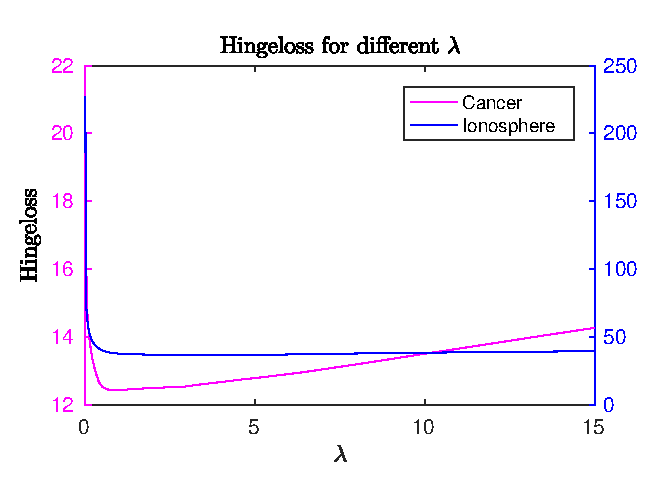
\includegraphics[width=\textwidth]{Pictures/Plots/lambda_vs_err_io_ca_final.eps}%
	\end{subfigure}
	\begin{subfigure}{0.49\textwidth}
		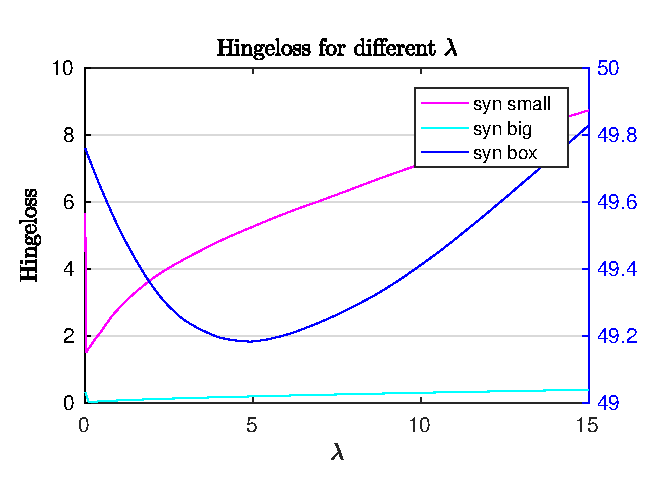
\includegraphics[width=\textwidth]{Pictures/Plots/lambda_vs_err_ss_sb_b5_final.eps}%
	\end{subfigure}
	\caption{Plots of the hingloss error for different $\lambda$ values. The figure on the right shows the plot for the \textup{\texttt{cancer}} (left axis) and \textup{\texttt{ionosphere}} (right axis) data sets. The blot on the left depicts the situation for the sythetic sets \textup{\texttt{syn small}}, \textup{\texttt{syn big}} (left axis) and \textup{\texttt{syn box}} (right axis).}%
	\label{fig_lambda_vs_err}%
\end{figure}


results

\begin{center}
\begin{table}[H]%
	\begin{tabular}{llcccc}
		\hline
    Data set & algorithm & 0.1 & 1 & 10 & 100 \\
		\hline
		\texttt{cancer} & Bundle & 1.0975 & 1.0974 & 1.0974 & 1.1341 \\
		 & Noll Bundle & 1.0974 & 1.0974 & 1.0974 & 1.0974 \\
		 &  fminsearch & 1.0974 & 1.0974 & 1.0974 & -10 \\
		 & fmindnb & 1.0974 \\
		\texttt{ionosphere} & Bundle & 2.6081 & 2.3108 & 0.3953 & 4.7401 \\
		 & Noll Bundle & 3.5386 & 3.6521 & 10 & 8.2773 \\
		 & fminsearch & 3.5104 & 3.5104 & 3.5104 & 3.5104 \\
		 & fminbnd & 3.5104 \\
		\texttt{syn small} & Bundle & 0.0337 & 0.031 & 0.0329& 0.03 \\
		 & Bundle Noll & 0.0323 & 0.0352 & 0.0352 & 0 \\
		 & fminsearch & 0.0346 & -0.1939 & -1.79 & -3.5673 \\
		 & fminbnd & 0.0346 \\
		\texttt{syn big} & Bundle & 0.1 & 1 & 10 & 100 \\
		 & Bundle Noll & 0.0099 & 0.0108 & 0.0109 & 0.0086 \\
		 & fminsearch & 0.0114 & -0.8748 & -0.8748 & -0.8748 \\
		 & fminbnd & 0.0206 & plot: 0.0114\\
		\texttt{syn box} & Bundle & 0.1 & 1 & 4.8486 & 4.45336 \\
		 & Bundle Noll & 0.1 & 1 & 4.2760 & 0 \\
		 & fminsearch & 4.8950 & 4.8950 & 4.8950 & 4.8950 \\
		 & fminbnd & 4.8950 \\
	\end{tabular}
	\caption{}
\end{table}
\end{center}

%times
%
%\begin{center}
%\begin{table}[H]%
	%\begin{tabular}{llcccc}
		%\hline
    %Data set & algorithm & 0.1 & 1 & 10 & 100 \\
		%\hline
		%\texttt{syn big} & Bundle Noll & 202 & 320 & 386 & 503 \\
		 %& fminsearch & 672 & 637 & 587 & 741 \\
		 %& fminbnd & 557
	%\end{tabular}
	%\caption{}
%\end{table}
%\end{center}
%
%sometimes says problem not convex, then negative values. Why??? Because tries negative lambda values in course of optimization and then it gets negative \\
%sometimes even for negative lambda in the end right solution \\
%can I find out why bundle methods so bad? \\
%try matlab method (smooth) with subgradient???
%
%
%
%%%%%%%%%%%%%%%%%%%%%%%%%%%%%%%%%%%%%%%%%%%%%%%%%%%%%%%%%%%%%%%%%%%%%%%%%%%%%%%%%%%%%%%%%%%%%%%%%%%%%%%%%%%%%%%%%%%%%%%%%%%%%%%%%%%%%%%%%%

%\subsubsection{Solution of the Bilevel Program}
%
%\textcolor{red}{ab hier: Theorie fehlt\\
%!!! notation - oder in prelininaries einfugen}
%%ingredients for bundle method
%
%To solve the given bilevel problem with the above presented nonconvex inexact bundle algorithm the algorithm jumps between the two levels. Once the inner level problems are solved for a given \(\lambda\) - this is possible with any QP-solver as the problems are convex - the bundle algorithm takes the outcome \(w\) and \(b\) and optimizes the hyper-parameter again.
%
%The difficulty with this approach is that the bundle algorithm needs one subgradient of the outer level objective function with respect to the parameter \(\lambda\). However to compute this subgradient also one subgradient of \(w\) and \(b\) with respect to \(\lambda\) has to be known.
%
%\textbf{The Differentiable Case}
%\textcolor{red}{example in differentiable case}\\
%Let us first assume that the outer and inner objective functions and \(w(\lambda)= \argmin \mathcal{L}_{low}(w,\lambda)\) are sufficiently often continuously differentiable to demonstrate the procedure of calculating the needed {(sub-)gradients}.
%
%Let \(\mathcal{L}_{upp}(w,\lambda)\) be the objective function of the outer level problem, where the variable \(b\) was left out for the sake of simplicity.
%To find an optimal hyper parameter \(\lambda\) given the input \(w\) the gradient \(g^{upp}_{\lambda}\) of \(\mathcal{L}_{upp}\) with respect to \(\lambda\) is needed in every iteration of the solving algorithm.
%In order to calculate this gradient the chain rule is used yielding
%
%\begin{equation*}
	%g^{upp}_{\lambda} = \left(\frac{\partial}{\partial w}\mathcal{L}_{upp}(w,\lambda) \right)^{\top}\frac{\partial w(\lambda)}{\partial\lambda}+\frac{\partial}{\partial \lambda}\mathcal{L}_{upp}(w,\lambda).
%\end{equation*}
%
%The challenge is here to find the term \(\frac{\partial w(\lambda)}{\partial\lambda}\) because 
%
%\[ \frac{\partial w}{\partial \lambda} \in \frac{\partial }{\partial \lambda} \argmin_{w} \mathcal{L}_{low}(w,\lambda). \]
%
%Assuming \(\mathcal{L}_{low}\) is twice continuously differentiable at the  optimal solution \(w^*\) of the lower level problem the optimality condition for any parameter \(\lambda_0 > 0\)
%
%\begin{equation}
	%0 = \frac{\partial}{\partial w}\mathcal{L}_{low}(w^*,\lambda_0)
%\label{opt_con}
%\end{equation}
%
%
%can be used to calculate the needed gradient in an indirect manner.
%
%In the differentiable case the theoretical framework for the following calculations is given by the implicit function theorem.
%
%\begin{theorem}[{c.f. \cite[chapter 3.4]{Koenigsberger2002}}]
	%Let \(F: U \times V \to Z \), \(U\in\R^m, V,Z\in \R^n \), be a \(\mathcal{C}^1\) mapping, \((x_0,y_0) \in U\times V\)  and \(F(x_0,y_0) = 0\). If the matrix \(\frac{\partial}{\partial y}F(x_0,y_0)\) is invertible, there exist neighborhoods \(U_0\subset U\) of \(x_0\) and \(V_0\subset V\) of \(y_0\) and a continuously differentiable mapping \(f:U_0 \to V_0\) with 
	%\begin{equation*}
	%F(x,y) = 0, (x,y)\in U_0\times V_0  \quad \Leftrightarrow \quad y = f(x), x\in U_0.
	%%\label{imp_fun_theo}
	%\end{equation*}
%\end{theorem}
%
%Identifying \(x \estimates \lambda\), \(y \estimates w\) and  \(F(x_0,y_0) \estimates \frac{\partial}{\partial w} \mathcal{L}_{low}(w^*,\lambda_0)\) and assuming \(\frac{\partial^2 }{\partial  w^2}\mathcal{L}_{low}(w^*,\lambda_0)\) is invertible this theorem provides the existence of the continuously differentiable function \(w(\lambda)\) whose gradient is needed. \\
%\textcolor{red}{what about the neighborhoods?}
%
%If the inner level loss function yields a linear optimality condition in \(w\) it is possible to calculate the gradient explicitly. This is for example the case for SVM loss functions with a squared one- or two-norm as given in problem (\ref{SVM_2}).
%The optimality condition can then be written as the linear system
%
%\begin{equation*}
	%H(\lambda)w = h(\lambda).
%\end{equation*}
%
%By taking the partial derivative with respect to \(\lambda\) on both sides of the system one gets
%
%\begin{equation*}
	%\frac{\partial H(\lambda)}{\partial \lambda}w+H(\lambda)\frac{\partial w}{\partial \lambda} = \frac{\partial h(\lambda)}{\partial  \lambda}.
%\end{equation*}
%
%If \(H(\lambda)\) is invertible for all \(\lambda \in \Lambda\) then the needed gradient is given by 
%
%\begin{equation*}
	%\frac{\partial w}{\partial \lambda} = H^{-1}(\lambda)\left(\frac{\partial h(\lambda)}{\partial \lambda}-\frac{\partial H(\lambda)}{\partial \lambda}w\right).
%\end{equation*}
%
%%\textcolor{red}{why H invertible??? - because we assume existence of \(w\)???}\\
%
%\textbf{The Nondifferentiable Case}
%\textcolor{red}{now for subgradients}
%
%In practice we cannot expect \(\mathcal{L}_{low}\) to satisfy such strong differentiability properties.
%It is therefore only assumed that \(\mathcal{L}_{low}\) is once continuously differentiable in \(w\). This assures that the optimality condition of the lower level problem is an equality like in (\ref{opt_con}).
%%If \(\mathcal{L}_{low}\) was only locally Lipschitz the optimality condition states that zero is part of the subgradient set  \(\partial \mathcal{L}_{low}(w^*,\lambda_0)\).  
%Contrary to the exemplary calculations from above in practice the second derivative \(\frac{\partial^2}{\partial w \partial \lambda} \mathcal{L}_{low}(w(\lambda),\lambda)\) however is not existent in this form, but a set of subgradients.
%
%
%
%\textcolor{red}{\textbf{Notation}}\\
%First the theoretical framework given to derive the results from above in the nondifferentiable case
%
%
%
%\textcolor{red}{An important result about Lipschitz functions is Rademacher's theorem which states that these functions are differentiable almost everywhere but on a set of Lebesgue measure zero\cite[Theorem 3.1]{Heinonen2004}. 
%Clarke deduces from this that the subdifferential at each of the nondifferentiable points is the convex hull of the limits of the sequence gradients a these points \cite[see Theorem 2.5.1]{Clarke1990}.}
%
%This motivates the multidimensional definition of Clake's generalized gradient 
%
%\textcolor{red}{
%\begin{definition}[{\cite[Definition 2.6.1]{Clarke1990}}]
	%\emph{generalized Jacobian}: \(F:\R^n \to \R^m\), with locally Lipschitz component functions \(F(x) = (f_1(x),...,f_m(x))\).\\
	%Denote generalized Jacobian by \(\partial F(x) = conv\left(\lim JF(x_i)|x_i\to x, x_i \notin \Omega_F \right) \) where \(\Omega_F\) is the set of nondifferentiable points of \(F\)
%\end{definition}
%(after that comes proposition with properties of \(\partial F\))}
%
%
%\textcolor{red}{To facilitate readability we use the following notation for the derivation of the nondifferentiable results.}
%
%The \emph{'partial' subdifferential} of a function \(f(a^*,b_0,c_0,...)\) at the point \(a^*\) with respect to one variable \(a\) when all other variables are fixed is denoted by 
%\begin{equation*}
	%\partial^{a} f(a^*,b_0,c_0,...).
%\end{equation*}
%
%A subgradient of this subdifferential is written \(g^{a} \in \partial^{a} f(a^*,b_0,c_0,...)\).
%
%Next step: show that chain rule is still valid in the nonsmooth case
%Chain rules for subdifferential \\
%
%\begin{theorem}[{\cite[Theorem 2.6.6]{Clarke1990}}]
	%Let \(f(x)=\phi(F(x))\), with the locally Lipschitz functions \(F: \R^n \to \R^m\) and \(\phi:\R^m \to \R\). Then \(f\) is locally Lipschitz and it holds
	%\begin{equation*}
		%\partial f \subset \text{conv}\left\{\partial \phi(F(x))\partial F(x)\right\}.
	%\end{equation*}
	%If in addition \(\phi\) is strictly differentiable at \(F(x)\), then equality holds.
%\end{theorem}
%
%\textcolor{red}{strictly differentiable: c.f. \cite[Theorem 9.17 and 9.18]{Rockafellar2009} locally Lipschitz continuous and at most one subgradient at the point in question (see also comment to Definition 91 in \cite{Rockafellar2009})}
%
%\begin{theorem}[c.f. {\cite[Theorem 7.1]{Rockafellar1985}}]
	%Let \(p(x) = f(F(x))\), where \(F:\R^n \to \R^d\) is locally Lipschitz and \(f:\R^d \to \R\) is lower semicontinuous. 
	%Assume \[\nexists y \in \partial^{\infty}f(F(\bar{x})), y \neq 0 \quad \text{with} \quad 0 \in y \partial F(\bar{x}). \]
	%Then for the sets 
	%\[ M(\bar{x}):= \partial f(F(\bar{x}))\partial F(\bar{x}), \quad M^{\infty}(\bar{x}):= \partial^{\infty}f(F(\bar{x}))\partial F(\bar{x}), \]
	%one has \(\hat{\partial}p(\bar{x}) \subset M(\bar{x})\) and \(\hat{\partial}^{\infty} p(\bar{x}) \subset M^{\infty}(\bar{x})\).
%\end{theorem}
%
%The main idea is to replace the inner level problem by its optimality condition
%
%
%\(\partial(w,b)\) means in this case that the subdifferential is taken with respect to the variables \(w\) and \(b\). \\
%-> theory for subdifferentials in more than one variable!!! \\
%
%For convex inner level problem this replacement is equivalent to the original problem.
%
%The difference to the approach described in \cite{Kunapuli2008} is that the problem is not smoothly replaced by its KKT conditions but only by this optimality condition. The weight vector \(w\) and bias \(b\) are treated as a function of \(\lambda\) and are optimized separately from this hyper-parameter.
%The reformulated bilevel problem becomes:
%
%\begin{align}
	%\begin{split}
	%\min_{w,\bm{b}} \quad &  \mathcal{L}_{hinge}(w,\bm{b}) = \frac{1}{T}\sum_{t=1}^T\frac{1}{|\mathcal{N}_t|}\sum_{i \in \mathcal{N}_t}{\max\left(1-y_i((w^t)^{\top}x-b_t),0\right)}\\
	%\text{subject to} \quad & \lambda > 0 \\
	%& \text{for } t = 1,...,T \\
	%& 0 \in \partial(w,b)\mathcal{L}_{low}(\lambda,w^t,b_t) \\
%\end{split}
%\label{SVM_opt_cond}
%\end{align}
%
%where \(\mathcal{L}_{low}\) can be the objective function of either of the two presented lower level problems.
%
%
%
%solve the inner level problem (quadratic problem in constrained case) by some QP solver \\
%put solution into upper level problem and solve it by using bundle method \\
%difficulty: subgradient is needed to build model of the objective function --> need subgradient \(\frac{\partial \mathcal{L}}{\partial \lambda}\) --> for this need \(\frac{\partial (W,b)}{\partial \lambda}\) \\
%but \((w,b)\) not available as functions -> only values
%
%Moore et al. \cite{Moore2011} describe a method for getting the subgradient from the KKt-conditions of the lower level problem:
%
%lower level problem convex -> therefore optimality conditions (some nonsmooth version -> source???) necessary and sufficient -> make ``subgradient'' of optimality conditions and then derive subgradient of w, b from this. \\
%---> what are the conditions? optimality condition Lipschitz? 
%
%Say (show) that all needed components are locally Lipschitz; state theorems about differentiability almost everywhere and convex hull of gradients gives set of subgradients\\
%introduce special notation (only for this section) and because of readability adopt ``gradient writing''
%
%Subgradients:
%\(\mathcal{G}_{upp,\lambda}, \mathcal{G}_{upp,w},\mathcal{G}_{upp,b}\) -> subgradients of outer objective \\
%\(g_w, g_b\) -> subgradient of w, b
%
%\[ final subgradient = \left(\mathcal{G}_{upp,w}(w,b,\lambda)\right)^{\top}g_w+\left(\mathcal{G}_{upp,b}(w,b,\lambda)\right)^{\top}g_b+\mathcal{G}_{upp,\lambda}(w,b,\lambda) 
%\label{subgr_upp}\]
%
%subgradients \(\mathcal{G}_{upp,...}\) easy to find (assumption that locally Lipschitz) -> in this application differentiable
%
%difficulty: find \(g_w, g_b\)
%important: optimality condition must be a linear system in \(w,b\) -> this is the case in this application
%\[ H(\lambda)\cdot (w,b)^{\top} = h(\lambda) \]
%
%find subgradients of each element (from differentiation rules follows)
%
%\[ \partial_{\lambda} H\cdot (w,b)^{\top} + H \cdot(\partial_{\lambda} w, \partial_{\lambda} b)^{\top} = \partial_{\lambda} h  \]
%
%solve this for \((w,b)\):
%\[ (\partial_{\lambda} w, \partial_{\lambda}b)^{\top} = H^{-1}\left(\partial_{\lambda}h-\partial_{\lambda} H \cdot(w,b)^{\top}\right) \]
%
%matrix \(H\) has to be inverted -> in the feature space so scalable with size of data set -> still can be very costly \cite{Moore2011}
%
%Applied to the two bilevel classification problems derived above, the subgradients have the following form:
%
%derivative of upper level objective:
%Notation: \(\delta_i := 1-y_i(w^{\top}x^i-b)\)
%
%\begin{align}
	%\partial_{w}\mathcal{L}_{upp}&= \frac{1}{T}\sum_{t=1}^T\frac{1}{\mathcal{N}_t}\sum_{i \in \mathcal{N}_t}{\left\{\begin{array}{cl} -y_ix^i & \text{if } \delta_i >0 \\ 0 & \text{if } \delta_i \leq 0 \end{array} \right.} \\
	%\partial_{b}\mathcal{L}_{upp}&= \frac{1}{T}\sum_{t=1}^T\frac{1}{\mathcal{N}_t}\sum_{i \in \mathcal{N}_t}{\left\{\begin{array}{cl} y_i & \text{if } \delta_i >0 \\ 0 & \text{if } \delta_i \leq 0 \end{array} \right.}
	%\end{align}
	%
	%here at the kink subgradient 0 is taken
%
%for hingequad: -> here subgradient \\
%optimality condition:
%\begin{align}
	%0 = \partial_{w}\mathcal{L}_{low} &= \lambda w+2\sum_{i \in \bar{\mathcal{N}_t}}{\left\{\begin{array}{cl} (1-y_i(w^{\top}x^i-b))(-y_ix^i) & \text{if } \delta_i >0 \\ 0 & \text{if } \delta_i \leq 0 \end{array} \right.} \\
	%0 = \partial_b\mathcal{L}_{low} &= 2\sum_{i \in \bar{\mathcal{N}_t}}{\left\{\begin{array}{cl} (1-y_i(w^{\top}x^i-b))(y_i) & \text{if } \delta_i >0 \\ 0 & \text{if } \delta_i \leq 0 \end{array} \right.}
	%\end{align}
	%
%subgradient??? is this smooth? with respect to \(\lambda\)
%\begin{align}
	%0 &= w+\lambda\partial_{\lambda}w+2\sum_{i \in \bar{\mathcal{N}_t}}{\left\{\begin{array}{cl} (-y_i(\partial_{\lambda}w^{\top}x^i-\partial_{\lambda}b))(-y_ix^i) & \text{if } \delta_i >0 \\ 0 & \text{if } \delta_i \leq 0 \end{array} \right.} \\
	%0 &= 2\sum_{i \in \bar{\mathcal{N}_t}}{\left\{\begin{array}{cl} (-y_i(\partial_{\lambda}w^{\top}x^i-\partial_{\lambda}b))(y_i) & \text{if } \delta_i >0 \\ 0 & \text{if } \delta_i \leq 0 \end{array} \right.}
%\end{align}
%
%From this the needed subgradients can be calculated via:
%
%\begin{equation}
	%2\cdot\begin{pmatrix} \frac{\lambda}{2}+\sum_{i \in \bar{\mathcal{N}_t}}{y_i^2x^i(x^i)^{\top}} & \sum_{i \in \bar{\mathcal{N}_t}}	{-y_i^2x^i} \\ \sum_{i \in \bar{\mathcal{N}_t}}{-y_i^2(x^i)^{\top}} & \sum_{i \in \bar{\mathcal{N}_t}}{y_i^2}\end{pmatrix}
	%\cdot \begin{pmatrix} \partial_{\lambda}w \\ \partial_{\lambda}b\end{pmatrix}
	%= \begin{pmatrix}-w \\ 0\end{pmatrix}
%\label{subgr_wb}
%\end{equation}
%
%for hinge not quad:
%
%not as much information in the subgradient/derivative
%
%similar calculation leads to 
%
%\begin{align}
	%\partial_{\lambda}w &= -\frac{w}{\lambda} \\
	%\partial_{\lambda}b &= 0
%\end{align}
%
%\textcolor{red}{does not work with just Hingeloss because set valued optimality condition --> have to find ``corresponding'' equation to the chosen subgradient --> do not know how}
%
%\subsubsection{Multi Group Model}
%
%Idea: different samples within the group have different have different quality --> put the samples with similar quality within one group --> give it its own \(\lambda_g\) such that the groups are weighted depending on their quality.
%
%two goals: better modleing and implicit information about the groups provided by the parameter \(\lambda_g\) -> small \(\lambda\) good quality, large \(\lambda\) bad quality???
%
%Examle: different people do same experiment; measure same data...
%
%\textbf{Model (Bilevel Problem)}
%
%
%for simplicity: all groups of same size; in all folds same number of elements of each group
%
%!! not possible to work with \(\lambda\) here, have to work with \(C\)-Formulation
%
%
%
%matrices for MATLAB calculations:
%
%\begin{equation*}
%\begin{split}
	%& \frac{1}{2} \langle x,Hx \rangle + h \\
	%& Ax \leq b
%\end{split}
%\end{equation*}
%
%\begin{equation}
	%H = \begin{pmatrix}
		%\mathbb{I}_{n\times n} \\
		%& 0 \\
		%& & 2 C \\
	%\end{pmatrix}
	%\in \R^{feat+1+J\max\{T-1,1\}G\times feat+1+J\max\{T-1,1\}G}
%\end{equation}
%
%\[ h = 0, \qquad A = \begin{pmatrix} -YX^{\top} & Y & -\mathbb{I}_{J\max\{T-1,1\}G \times J\max\{T-1,1\}G} \\ \end{pmatrix},  \qquad b = -\mathtt{ones}(J\max\{T-1,1\}G,1) \] 
%
%with \(C = [\underbrace{c_1,...,c_1}_{J\max\{T-1,1\} \text{ times}},c_2,...,c_2,...,c_G,...,c_G]^{\top}\).
%
%\textbf{Derivatives}
%
%overall gradient:
	%\[ \frac{\textup{d}\mathcal{L}_{upp}}{\textup{d}\lambda} = {\underbrace{\frac{\partial \mathcal{L}_{upp}}{\partial (w,b)}}_{\in \R^{n+1}}} ^{\top} \underbrace{\frac{\partial (w,b)}{\partial \lambda}}_{\in \R^{n+1 \times G}} \in \R^G\]
%
%
%gradient outer level objective: 
	%\[ \frac{\partial \mathcal{L}_{upp}}{\partial w} = \frac{1}{T}\sum_{t=1}^T\frac{1}{|\mathcal{N}_t|}\sum_{i \in \mathcal{N}_t} \delta_i \left( -y_i x^i\right) \in \R^n\]
	%
	%\[ \frac{\partial \mathcal{L}_{upp}}{\partial b} = \frac{1}{T}\sum_{t=1}^T\frac{1}{|\mathcal{N}_t|}\sum_{i \in \mathcal{N}_t} \delta_i y_i \in \R\]
	%
	%\[ \delta_i = \left\{ \begin{array}{cl} 1 & \text{if } 1-y_i\left(\Langle w,x^i\Rangle-b\right) > 0 \\
		%0 & \text{else}\end{array} \right.\]
%
%
%in MATLAB: 
	%\[ \frac{\partial \mathcal{L}_{upp}}{\partial w} = \frac{1}{T}\texttt{sum}(-\texttt{bsxfun}(\texttt{@times},X,\texttt{delta}.*Y) ,2) \in \R^n\]
	%
	%\[ \frac{\partial \mathcal{L}_{upp}}{\partial b} = \frac{1}{T}\texttt{sum}(\texttt{delta}.*Y ,1) \in \R\]
	%
	%
%gradient lower level objective:\\
%first optimality conditions \(0 = \frac{\partial \mathcal{L}_{low}}{\partial w}, 0 = \frac{\partial \mathcal{L}_{low}}{\partial b}\):
	%\[ 0 = {\sum_{g = 1}^G(\lambda_g}w) + 2\sum_{i \in \bar{\mathcal{N}}_t}\delta_i \left\{1-y_i\left(\Langle w,x^i\Rangle -b\right) \right\}(-y_ix^i) \in \R^n \]
		%
	%\[0 = 2\sum_{i \in \bar{\mathcal{N}}_t}\delta_i \left\{1-y_i\left(\Langle w,x^i\Rangle -b\right) \right\}(y_i) \in \R \]
	%
	%derivatives with respect to \(\lambda_g, g = 1,...,G\), then \(\in \R^{n+1 \times G}\)
	%
	%write one column of the matrix \(\in \R^{n+1}\) \(\to\) \(G\) such columns:
	%
	%\[ 0 = w + \lambda_g\frac{\partial w}{\partial \lambda_g} + 2 \sum_{i \in  \bar{\mathcal{N}}_t} \delta_i \left(y_i^2x^i(x^i)^{\top}\frac{\partial w}{\partial \lambda_g} - y_i^2x^i \frac{\partial b}{\partial \lambda_g}\right) \in \R^n \]
	%
	%\[ 0 = 2\sum_{i \in  \bar{\mathcal{N}}_t} \delta_i \left(-y_i^2(x^i)^{\top} \frac{\partial w}{\partial \lambda_g} + y_i^2 \frac{\partial b}{\partial \lambda_g}\right) \in \R\] 
%
%
	%rewrite to calculate \([\partial w / \partial \lambda, \partial b / \partial \lambda]^{\top} \in \R^{n+1 \times G}\) \(\to\) have to calculate every column of this matrix on its own \\
	%solve \(G\) times this system of equations
	%
	%\[ 2\begin{pmatrix} \frac{\lambda_g}{2}\mathbb{I}+\sum_{i \in  \bar{\mathcal{N}}_t}{\delta_i(y_i^2x^i(x^i)^{\top})} &  \sum_{i \in  \bar{\mathcal{N}}_t} \delta_i (- y_i^2x^i )	\\
	%\sum_{i \in  \bar{\mathcal{N}}_t} \delta_i (-y_i^2(x^i)^{\top}) & \sum_{i \in  \bar{\mathcal{N}}_t} \delta_i (y_i^2 )
	%\end{pmatrix} 
	%\begin{pmatrix}	\frac{\partial w}{\partial \lambda_g} \\ \frac{\partial b}{\partial \lambda_g}
	%\end{pmatrix} 
	%= \begin{pmatrix} -w \\ 0	\end{pmatrix} \]
%









